\chapter{Secure Cloud Deployment Framework (SCDF)}
\label{chap:third}

\ifpdf
    \graphicspath{{Chapter3/Figures/PNG/}{Chapter3/Figures/PDF/}{Chapter3/Figures/}}
\else
    \graphicspath{{Chapter3/Figures/EPS/}{Chapter3/Figures/}}
\fi

% ----------------------------------------------------------
\section{Chapter Overview and Positioning}
\label{sec:chapter3_overview}

This chapter presents the Secure Cloud Deployment Framework (SCDF)---a structured, evidence-driven approach tailored for Small and Medium Enterprises (SMEs) to deploy cloud infrastructure securely, with emphasis on operational feasibility under real-world constraints.

Cloud adoption offers SMEs scalability, cost efficiency, and flexibility; however, security risks and skill gaps remain critical concerns that commonly hinder secure implementation and long-term operations. According to cybersecurity analyses focused on SMEs, fundamental challenges such as limited budgets, scarcity of specialized expertise, and low security awareness significantly increase vulnerability to threats and misconfigurations in cloud environments. This is affirmed by the European Union Agency for Cybersecurity (ENISA), which notes that SMEs frequently lack clear, tailored guidance suited to their unique operational context, and that such guidance is essential for safe cloud adoption and risk management \citep{ENISA2015CloudSecurityGuideSMEs}.

SCDF arises from a juxtaposition of two realities:

\begin{itemize}
    \item \textbf{Operational necessity:} Cloud platforms are increasingly essential for SME digital transformation, supporting everything from basic infrastructure to business continuity.
    
    \item \textbf{Security challenge:} SMEs often operate without formal cybersecurity governance, dedicated teams, or enterprise-grade tools, yet face the same spectrum of threats that larger organizations do---including misconfigurations, identity compromise, and ransomware exposure.
\end{itemize}

This chapter translates systematic insights from the literature into SCDF---a framework that operationalizes key security principles into actionable and verifiable actions suitable for SMEs on Infrastructure-as-a-Service (IaaS) platforms. Rather than aiming for comprehensive enterprise compliance (e.g., ISO/IEC 27001 certification), SCDF focuses on deployable minimum viable security mechanisms that measurably reduce risk while preserving accessibility and cost-effectiveness. SCDF is informed by cloud-specific guidance (e.g., ISO/IEC 27017) to support pragmatic control selection and responsibility assignment without requiring formal certification \citep{WikipediaISOIEC27017}.

% ----------------------------------------------------------
\section{Scope Definition and Applicability Boundaries}
\label{sec:scope_definition}

This section defines the scope of SCDF's applicability and delineates the boundaries of what the framework does and does not address. These definitions ensure that SCDF's recommendations remain realistic, actionable, and relevant for the intended user group---Small and Medium Enterprises (SMEs) operating in cloud environments with distinct constraints.

\subsection{Target SME Profile}
\label{subsec:target_sme_profile}

SCDF is intended primarily for SMEs that share a set of organizational, technical, and economic characteristics common in developing and resource-constrained environments. SME research highlights that such organizations often adopt cloud computing to overcome infrastructural limitations and cost barriers, but concurrently struggle with security and privacy concerns, limited technical experience, and minimal governance structures. These challenges contribute to hesitancy in cloud adoption despite strong perceived benefits such as scalability and cost efficiency \citep{ENISA2015CloudSecurityGuideSMEs,Erdogan2023CybersecurityAwareness}.

An SME appropriate for SCDF typically exhibits the following features:

\begin{itemize}
    \item \textbf{Organizational scale:} Fewer than 250 employees with limited or no dedicated cybersecurity personnel, making specialized security teams impractical.
    
    \item \textbf{Technical capacity:} Reliance on generalist IT staff, outsourced IT support, or ad-hoc technical management without specialized cybersecurity training. This lack of in-house expertise is widely recognized as a critical barrier to secure cloud adoption in SMEs.
    
    \item \textbf{Cloud consumption model:} Primary use of Infrastructure-as-a-Service (IaaS) offerings, including virtual machines, storage, and basic networking, rather than complex platform or container ecosystems.
    
    \item \textbf{Economic constraints:} High cost sensitivity and preference for cost-effective or open-source tooling, as is common among SMEs evaluating cloud security tools.
    
    \item \textbf{Operational environment:} Unreliable connectivity and limited administrative bandwidth, common in developing regions where cloud adoption is essential yet operational challenges remain.
\end{itemize}

This SME profile reflects a modal class of organizations that significantly benefit from cloud computing but face constraints that make conventional enterprise-scale security frameworks impractical.

\subsection{Explicit Exclusions}
\label{subsec:explicit_exclusions}

To maintain realism and utility, SCDF explicitly excludes the following objectives and control categories. These exclusions are not oversights but intentional boundaries grounded in normative research on SMEs' limited capacity for exhaustive security frameworks and compliance activities:

\begin{itemize}
    \item \textbf{Formal certification pursuit:} SCDF does not provide the comprehensive control documentation or audit structures required to earn certifications such as ISO/IEC 27001, SOC 2, or equivalent compliance attestations. While such standards offer valuable guidance, they often require significant governance resources that exceed the operational capacity of target SMEs. SME guidance specifically emphasizes that organizations cannot always implement full enterprise-grade frameworks due to time, expertise, and financial constraints.
    
    \item \textbf{Enterprise-scale Zero Trust architectures:} Full Zero Trust implementations---involving pervasive identity attestation, micro-segmentation, and continuous contextual authorization---demand advanced tooling and governance structures typically outside SME capacity at initial phases. SCDF instead incorporates risk-appropriate identity and access principles that embody Zero Trust philosophies without architectural complexity.
    
    \item \textbf{Dedicated Security Operations Center (SOC) capabilities:} Round-the-clock threat hunting, specialist incident response teams, and continuous human monitoring exceed the operational budget and personnel availability of most SMEs. SCDF emphasizes automated detection with prioritized alerts to balance visibility with resource expense.
    
    \item \textbf{Provider obligation substitution:} SCDF recognizes but does not replace the cloud provider's responsibilities for physical infrastructure, hypervisor integrity, and connectivity backbone security. The framework operates strictly within the shared responsibility model and leaves provider-side assurances to established cloud contractual and architectural practices.
\end{itemize}

By clearly defining what SCDF does not aim to achieve, the framework maintains focus, feasibility, and applicability for its intended users without overpromising outcomes inconsistent with SME realities.

% ----------------------------------------------------------
\section{Derivation of Framework Requirements from SLR Findings}
\label{sec:derivation_requirements}

The design of the Secure Cloud Deployment Framework (SCDF) is systematically derived from evidence synthesized in the Systematic Literature Review (SLR) presented in Chapter 2. This derivation translates recurring themes in cloud security literature --- particularly those relating to SME constraints and practical threat landscapes --- into actionable framework requirements that address real-world risk vectors. Contemporary systematic reviews of cloud security identify a range of threats and mitigation strategies that are directly relevant to SMEs. These include identity and access vulnerabilities, misconfigurations, DDoS and malware threats, data breaches, and the need for security awareness and vulnerability management techniques such as IAM, SIEM, and encryption \citep{Milhem2025integrated,Al2023Security}. Importantly, multiple reviews also highlight that cloud misconfigurations --- incorrect permissions, weak IAM settings, overly permissive networks, and reduced monitoring --- are consistently among the top causes of cloud security incidents and exploited vulnerabilities \citep{Gibreel2023Factors,Sabah2024Cloud}.

The SCDF requirements are mapped to these empirical findings through a structured goal-to-requirement transformation, as shown in Table~\ref{tab:slr_to_requirements}. Each requirement targets measurable improvement in areas identified repeatedly across SLR outputs.

\begin{table}[htbp]
    \centering
    \caption{Mapping SLR Findings to SCDF Requirements}
    \label{tab:slr_to_requirements}
    \resizebox{\textwidth}{!}{%
    \begin{tabular}{|p{5cm}|p{4cm}|p{5cm}|}
        \hline
        \textbf{SLR Finding} & \textbf{Identified Constraint} & \textbf{SCDF Requirement} \\
        \hline
        Misconfiguration is a prominent contributor to cloud security issues (permissions, network ACLs, APIs) \citep{Gibreel2023Factors,Chen2023Securing}. & Limited SME expertise and human errors & Secure-by-default baselines and automated configuration validation procedures \\
        \hline
        Identity and access weaknesses (account hijacking, weak credentials, privilege misuse) \citep{Al2023Security,Trigueros2024Security}. & Lack of trained security personnel and complex IAM & Constrained guided workflows for IAM and enforced multi-factor identity controls \\
        \hline
        High threat diversity --- from malware to data breaches to denial of service attacks \citep{Tanimu2023Review,Gupta2023Deep}. & Insufficient threat visibility and response capability & Incremental monitoring controls with verified alerting thresholds and prioritized response \\
        \hline
        Cost and complexity inhibit adoption of enterprise-grade security tools \citep{Skafi2020Factors,Wilson2015Enablers,Sayginer2021Multi}. & Severe budget limitations and tooling barriers & Explicit preference for OSS, freemium tools, and cloud-native controls with trade-off documentation \\
        \hline
        High variability in cloud deployments (providers, architectures, workloads) \citep{Rashid2024Analysis,Abdulsalam2023Security}. & Low operational applicability of generic frameworks & Concrete control mapping with provider-agnostic and provider-specific implementation notes and step-by-step workflows \\
        \hline
        SLA, governance, and formal risk management are often absent in SMEs \citep{Chan2023Digital,Matias2019Cloud}. & Absence of formal governance structures & Lightweight governance templates with accountability roles and risk acceptance logs \\
        \hline
    \end{tabular}%
    }
\end{table}

\subsection{Validation of Requirements}

Each derived requirement addresses a documented failure mode from the literature. For example, the requirement for secure-by-default baselines responds directly to findings that SMEs frequently deploy with default configurations due to lack of implementation guidance \citep{Milhem2025integrated,Gibreel2023Factors}. Similarly, the preference for open-source tooling addresses the economic constraints identified across multiple regional studies \citep{Skafi2020Factors,Wilson2015Enablers,Sayginer2021Multi}.

% ----------------------------------------------------------
\section{Design Principles and Trade-Off Rationale}
\label{sec:design_principles}

This section establishes the foundational design principles that govern the Secure Cloud Deployment Framework (SCDF) and explains the explicit trade-offs made to balance security effectiveness with deployability for Small and Medium Enterprises (SMEs). Each principle is grounded in current cloud security understanding and reflects patterns observed in cloud security literature and practical SME guidance.

Cloud security frameworks universally emphasize the need for risk prioritization, control consistency, and measurable outcomes \citep{Chen2023Securing,Al2023Security}. For SMEs with limited security expertise and resources, SCDF's design principles adapt these general concepts into a pragmatic, incremental, and outcome-oriented approach that avoids over-prescription and unnecessary complexity. This aligns with guidance from SME-focused cloud security frameworks, which recommend simplified risk assessment and control implementation tailored to organizational capacity rather than enterprise-grade compliance mandates \citep{Skafi2020Factors,Wilson2015Enablers}.

\subsection{Core Design Principles}
\label{subsec:core_principles}

Each SCDF principle reflects a design trade-off between ideal security constructs and the practical realities SMEs face. These principles are intended to guide both what SMEs should implement and how they should approach security progression in cloud environments.

\begin{enumerate}
    \item \textbf{Risk-Driven Prioritization}
    
    In cloud environments, certain controls offer disproportionately higher security impact relative to effort --- especially in SME contexts where attack vectors such as identity compromise or misconfigurations are common. For this reason, SCDF orders controls by risk frequency and impact, emphasizing identity, network, and configuration hardening before more advanced areas.
    
    This principle aligns with risk-focused guidance in cloud security research that highlights prioritized mitigation of identity and access threats and misconfiguration avoidance \citep{Gibreel2023Factors,Trigueros2024Security}. It also resonates with the Identify and Protect components of established cybersecurity models (e.g., NIST CSF), which prioritize risk assessment and protective measures early in a security lifecycle.
    
    \item \textbf{Minimal Viable Security}
    
    SCDF aims for minimum viable security, defined as the smallest set of effective controls that reduce critical risks to an acceptable level. Rather than seeking exhaustive control coverage, this principle favors practical sufficiency --- implementing just enough security that significantly reduces risk without overwhelming limited operational capacity.
    
    SME cloud security literature consistently observes that over-complex frameworks discourage adoption, especially when SMEs lack security staff \citep{Chan2023Digital,Matias2019Cloud}. This principle echoes the Secure by Design approach, where security is built into system configurations early and in a targeted manner rather than patched in later reactively \citep{Rashid2024Analysis}.
    
    \item \textbf{Automation as Compensation, Not Replacement}
    
    Automated tooling (e.g., configuration scanners, cloud posture management) helps address skill gaps by enforcing consistency and reducing drift, but it does not eliminate the need for human oversight. SCDF leverages automation to enforce repeatable validation and routine tasks (e.g., baseline assessment), yet explicitly retains human judgment for strategic decisions and incident responses.
    
    Modern cloud monitoring paradigms and continuous threat exposure approaches emphasize that automation improves detection and response efficiency but must be paired with human risk decisions \citep{Tanimu2023Review,Gupta2023Deep}.
    
    \item \textbf{Incremental Maturity}
    
    Reflecting the incremental nature of security maturity, SCDF defines four deployment phases that build sequentially. This allows SMEs to achieve incremental risk reduction while learning and allocating resources gradually.
    
    Incremental maturity mirrors continuous monitoring and maturity models in cloud security best practices, proposing progressive improvements rather than all-at-once adoption \citep{Abdulsalam2023Security,Sabah2024Cloud}.
    
    \item \textbf{Provider Agnosticism with Pragmatic Exceptions}
    
    SCDF's controls are designed to be implementable across multiple IaaS platforms, but vendor-specific native controls are permitted when they reduce cost and complexity without compromising security outcomes. This reflects the practical reality that SMEs often prefer cloud-native services for integrated functionality and minimal operational overhead.
    
    SME guidance acknowledges that cloud provider native tools can be leveraged effectively to meet baseline security needs with lower cost and integration effort \citep{Sayginer2021Multi,Milhem2025integrated}.
\end{enumerate}

\subsection{Explicit Trade-Offs}
\label{subsec:explicit_tradeoffs}

Deploying security within resource-constrained organizations requires explicit acknowledgement of trade-offs. The following articulates the key tensions SCDF resolves:

\textbf{Breadth vs Deployability}

SCDF deliberately limits coverage to the most impactful controls initially, postponing niche or advanced capabilities to later phases. The rationale is that controls which remain unimplemented due to complexity offer no protection at all; partial implementation of priority controls enhances risk reduction meaningfully. This trade-off parallels cloud security best-practice guidance that promotes prioritization of high-impact controls (e.g., IAM, logging) before expanding to less impactful domains \citep{Chen2023Securing,Rashid2024Analysis}.

\textbf{Advanced vs Baseline Protection}

Sophisticated detection and analytics (e.g., behavior-based analytics, custom detection rules) are valuable, but are deferred until baseline security, monitoring, and hardening are stable. SCDF prioritizes foundational protections (MFA, least-privilege access, default-deny networking) before introducing complex monitoring that demands more expertise. Cloud monitoring best practices emphasize foundational logging and SIEM readiness before layering advanced analytics for threat hunting \citep{Tanimu2023Review,Gupta2023Deep}.

\textbf{Vendor Neutrality vs Pragmatic Efficiency}

While the framework promotes core principles that are conceptual and provider-agnostic, it endorses the use of vendor-native tools where they are demonstrably easier to implement and maintain. This reflects guidance advocating the pragmatic use of cloud-native security capabilities alongside open-source tooling for SMEs \citep{Sayginer2021Multi,Skafi2020Factors}.

\subsection{Summary of Design Principles and Trade-Offs}
\label{subsec:design_summary}

The design of SCDF explicitly balances effectiveness and practicality. It embeds core best practices from cloud security literature into a framework that assumes limited resources, limited expertise, and the need for measurable outcomes. The principles are not theoretical ideals but a composition of documented patterns of risk and mitigation strategies validated in cloud security guidance and empirical studies \citep{Al2023Security,Gibreel2023Factors,Trigueros2024Security}.

% ----------------------------------------------------------
\section{Conceptual Structure of the SCDF}
\label{sec:conceptual_structure}

The Secure Cloud Deployment Framework (SCDF) organizes its guidance into a three-layer architecture that aligns with established information security principles --- separating governance, control implementation, and operations. This layered approach mirrors the defense-in-depth architecture common in cloud and IT security, where multiple, complementary layers of protection are applied to mitigate threats and reduce attack surface \citep{Chen2023Securing,Al2023Security}.

A layered structure helps SMEs reason about who decides (governance), what is implemented (controls), and how it runs daily (operations), without conflating strategic oversight with tactical execution.

\subsection{Framework Layers}
\label{subsec:framework_layers}

SCDF is structured into the following three core layers, as illustrated in Figure~\ref{fig:scdf_layers_revised}.

\begin{figure}[htbp]
    \centering
    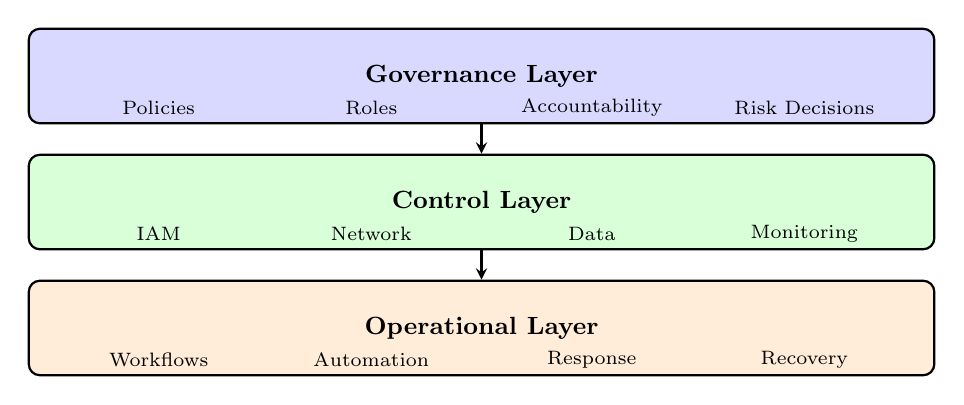
\begin{tikzpicture}[
        layer/.style={rectangle, rounded corners, minimum width=11.5cm, minimum height=1.2cm, text centered, font=\small\bfseries, draw, thick},
        item/.style={font=\scriptsize, align=center},
        arrow/.style={->, >=stealth, thick}
    ]
        \node[layer, fill=blue!15] (gov) at (0,3.2) {Governance Layer};
        \node[item] at (-4.1,2.8) {Policies};
        \node[item] at (-1.4,2.8) {Roles};
        \node[item] at (1.4,2.8) {Accountability};
        \node[item] at (4.1,2.8) {Risk Decisions};

        \node[layer, fill=green!15] (ctrl) at (0,1.6) {Control Layer};
        \node[item] at (-4.1,1.2) {IAM};
        \node[item] at (-1.4,1.2) {Network};
        \node[item] at (1.4,1.2) {Data};
        \node[item] at (4.1,1.2) {Monitoring};

        \node[layer, fill=orange!15] (ops) at (0,0) {Operational Layer};
        \node[item] at (-4.1,-0.4) {Workflows};
        \node[item] at (-1.4,-0.4) {Automation};
        \node[item] at (1.4,-0.4) {Response};
        \node[item] at (4.1,-0.4) {Recovery};

        \draw[arrow] (gov) -- (ctrl);
        \draw[arrow] (ctrl) -- (ops);
    \end{tikzpicture}
    \caption{SCDF Three-Layer Architecture (Governance, Controls, Operations)}
    \label{fig:scdf_layers_revised}
\end{figure}

\begin{enumerate}
    \item \textbf{Governance Layer}
    
    The Governance Layer establishes policies, roles, and accountability mechanisms that guide all other security activities. It answers strategic questions such as:
    \begin{itemize}
        \item What security objectives align with the SME's business needs?
        \item Who is responsible for approving risk decisions?
        \item What policies govern acceptable use, exceptions, and escalation paths?
    \end{itemize}
    
    This layer is essential for clarifying decision authority, documenting risk acceptance, and ensuring that operational activities are anchored in organizational intent rather than ad-hoc technician decisions. In established cloud and cybersecurity frameworks, governance is recognized as foundational and prerequisite to effective control implementation --- guiding risk appraisal and policy enforcement \citep{Gibreel2023Factors,Trigueros2024Security}.
    
    \item \textbf{Control Layer}
    
    The Control Layer translates governance directives into technical and procedural controls that protect the SME's cloud environment. It includes:
    \begin{itemize}
        \item \textbf{Identity and Access Management (IAM):} Restricting access via secure authentication and least-privilege policies, a control repeatedly identified as foundational in cloud security literature \citep{Tanimu2023Review}.
        \item \textbf{Network Security:} Firewalls, security groups, and segmentation concepts (including defense-in-depth patterns) to limit unauthorized access \citep{Rashid2024Analysis}.
        \item \textbf{Data Security:} Use of encryption and access policies to protect sensitive assets.
        \item \textbf{Monitoring and Logging:} Mechanisms for detecting anomalous behaviors, configuration changes, and potential compromise.
    \end{itemize}
    
    According to cloud security control taxonomies, such layered controls are essential to protect data, compute, and network assets from evolving threats and maintain confidentiality, integrity, and availability \citep{Abdulsalam2023Security,Sabah2024Cloud}.
    
    The Control Layer embodies the what --- the set of safeguards that enforce governance policies in the cloud environment.
    
    \item \textbf{Operational Layer}
    
    The Operational Layer defines executable workflows, automation scripts, and response procedures that translate controls into daily practice. This includes:
    \begin{itemize}
        \item Routine security configuration validation
        \item Scheduled automated scans
        \item Alert triage and escalation playbooks
        \item Backup execution and recovery rehearsals
    \end{itemize}
    
    The Operational Layer represents how controls are executed on a recurring basis, enabling SMEs to operationalize security through repeatable and measurable actions. Cloud security best practices emphasize that controls without operational execution --- such as regular scans, alerts, or backups --- achieve little. Embedding detection and response in day-to-day practice is essential for actual risk reduction rather than theoretical compliance \citep{Gupta2023Deep,Milhem2025integrated}.
\end{enumerate}

\subsubsection{Layer Interaction Model}
\label{subsubsec:layer_interaction}

The three layers interact through top-down direction and bottom-up feedback:
\begin{itemize}
    \item \textbf{Governance informs Controls:} Governance policies and risk decisions define which controls must be implemented and enforced.
    \item \textbf{Controls shape Operations:} Controls define the operational activities required; operations execute and validate these controls.
    \item \textbf{Operations feed into Governance:} Operational outcomes (e.g., metrics, incident reports) inform governance reviews and policy updates, ensuring continuous improvement.
\end{itemize}

\begin{figure}[htbp]
    \centering
    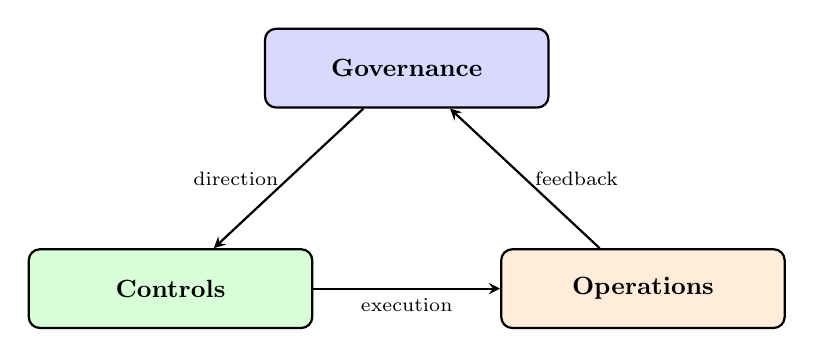
\begin{tikzpicture}[
        node/.style={rectangle, rounded corners, minimum width=3.6cm, minimum height=1cm, draw, thick, text centered, font=\small\bfseries},
        arrow/.style={->, >=stealth, thick}
    ]
        \node[node, fill=blue!15] (g) at (0,1.8) {Governance};
        \node[node, fill=green!15] (c) at (-3,-1) {Controls};
        \node[node, fill=orange!15] (o) at (3,-1) {Operations};

        \draw[arrow] (g) -- node[left, font=\scriptsize]{direction} (c);
        \draw[arrow] (c) -- node[below, font=\scriptsize]{execution} (o);
        \draw[arrow] (o) -- node[right, font=\scriptsize]{feedback} (g);
    \end{tikzpicture}
    \caption{Layer Interaction Cycle: Direction, Execution, and Feedback}
    \label{fig:layer_interaction_cycle}
\end{figure}

This feedback loop echoes iterative cybersecurity lifecycle recommendations found in frameworks like continuous threat exposure management (CTEM), where ongoing validation and adaptation are key to maintaining resilience \citep{Skafi2020Factors,Wilson2015Enablers}.

\subsection{Deployment Phases}
\label{subsec:deployment_phases}

Implementation follows four sequential phases, each building on the previous, as shown in Figure~\ref{fig:deployment_phases}.

\begin{figure}[htbp]
    \centering
    \begin{tikzpicture}[
        phase/.style={rectangle, rounded corners, minimum width=3cm, minimum height=1.5cm, text centered, align=center, font=\small\bfseries, draw, thick},
        arrow/.style={->, >=stealth, very thick},
        focus/.style={font=\scriptsize, align=center, text width=3cm}
    ]
        % Phase boxes
        \node[phase, fill=blue!15] (p1) at (0,0) {Phase 1\\Baseline};
        \node[phase, fill=green!15] (p2) at (4,0) {Phase 2\\Hardening};
        \node[phase, fill=orange!15] (p3) at (8,0) {Phase 3\\Monitoring};
        \node[phase, fill=red!15] (p4) at (12,0) {Phase 4\\Recovery};
        
        % Arrows
        \draw[arrow] (p1) -- (p2);
        \draw[arrow] (p2) -- (p3);
        \draw[arrow] (p3) -- (p4);
        
        % Focus areas
        \node[focus, below=0.5cm of p1] {Identity\\Network\\Logging};
        \node[focus, below=0.5cm of p2] {Config Standards\\Vulnerability Mgmt\\Access Control};
        \node[focus, below=0.5cm of p3] {SIEM\\Alerting\\Audit};
        \node[focus, below=0.5cm of p4] {Backups\\Recovery Plans\\Continuity};
        
        % Risk reduction indicator
        \node[above=1cm of p2, font=\small, align=center] {\textbf{Risk Reduction Priority}\\(Highest \textrightarrow Lower)};
    \end{tikzpicture}
    \caption{SCDF Four-Phase Deployment Sequence}
    \label{fig:deployment_phases}
\end{figure}

Implementation follows four sequential phases, each building on the previous:

\begin{enumerate}
    \item \textbf{Phase 1: Baseline Establishment} --- Secure the foundation including identity management, network boundaries, and initial logging.
    
    \item \textbf{Phase 2: Risk Hardening} --- Implement configuration standards, vulnerability management, and access controls.
    
    \item \textbf{Phase 3: Monitoring and Detection} --- Deploy continuous monitoring, alerting, and audit capabilities.
    
    \item \textbf{Phase 4: Backup, Recovery, and Continuity} --- Ensure resilience through automated backups and documented recovery procedures.
\end{enumerate}

These phases are ordered by risk reduction per unit effort. Phase 1 controls (identity and network) address the highest-impact threat vectors and therefore take priority over Phase 4 controls (backup and recovery), despite the importance of both \citep{Brandefense2025CloudSecuritySMEs,InterceptAzureSecurityEbook,Scrut2022CloudSecurityMonitoring}.

\begin{figure}[htbp]
    \centering
    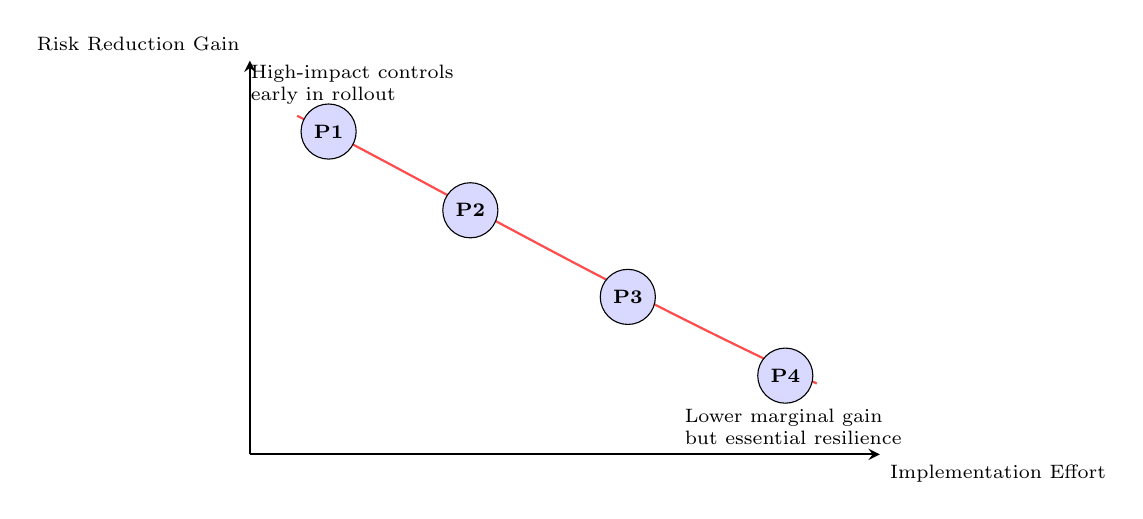
\begin{tikzpicture}[
        >=stealth,
        axis/.style={->, thick},
        phase/.style={circle, draw, fill=blue!15, minimum size=7mm, inner sep=0pt, font=\scriptsize\bfseries}
    ]
        % Axes
        \draw[axis] (0,0) -- (8,0) node[below right, font=\scriptsize] {Implementation Effort};
        \draw[axis] (0,0) -- (0,5) node[above left, font=\scriptsize] {Risk Reduction Gain};

        % Curve
        \draw[thick, red!70] (0.6,4.3) .. controls (2.2,3.5) and (4.4,2.2) .. (7.2,0.9);

        % Phase points
        \node[phase] (p1) at (1.0,4.1) {P1};
        \node[phase] (p2) at (2.8,3.1) {P2};
        \node[phase] (p3) at (4.8,2.0) {P3};
        \node[phase] (p4) at (6.8,1.0) {P4};

        \node[font=\scriptsize, align=left] at (1.3,4.7) {High-impact controls\\early in rollout};
        \node[font=\scriptsize, align=left] at (6.9,0.35) {Lower marginal gain\\but essential resilience};
    \end{tikzpicture}
    \caption{Indicative Risk Reduction per Unit Effort Across SCDF Phases}
    \label{fig:risk_effort_curve}
\end{figure}

\subsection{Phase Advancement Criteria}
\label{subsec:phase_advancement_criteria}

To ensure objective and measurable progression through the SCDF deployment phases, SCDF adopts a \textbf{hybrid advancement model} (Option C) that combines minimum tool completion requirements with quantitative risk metric thresholds. This approach mitigates the limitations of checklist-only methods---which risk superficial compliance---and metric-only methods---which risk advancement without foundational controls present.

This hybrid model reflects best practices in security assessment frameworks that utilize Goal-Question-Metrics (GQM) approaches and risk-based evaluation to quantitatively assess security posture and maturity levels tailored to SMEs. By requiring both control presence and demonstrated risk reduction, SCDF ensures that advancement represents genuine security improvement rather than administrative compliance.

Each advancement step requires:
\begin{enumerate}
    \item Completion of essential controls and tooling appropriate for that phase, and
    \item Achievement of quantitative risk reduction or maturity thresholds as measured by accepted security assessment tools and methodologies.
\end{enumerate}


\subsubsection{Phase 1 $\rightarrow$ Phase 2 Advancement Criteria}
\label{subsubsec:p1_to_p2}

An SME may advance to Phase 2 (Risk Hardening) only when:

\begin{enumerate}
    \item \textbf{Mandatory Controls Are Implemented}
    \begin{itemize}
        \item Identity and Access Management (IAM) policies configured per least-privilege principles.
        \item Multi-Factor Authentication (MFA) enabled for all privileged accounts and administrative access.
        \item Network security groups or equivalent (e.g., firewall rules) deployed and attached to all compute instances.
    \end{itemize}
    
    \item \textbf{Quantitative Evidence of Configuration Risk Reduction}
    \begin{itemize}
        \item A cloud posture assessment (e.g., Prowler, ScoutSuite, or equivalent) shows \textbf{no critical findings} in identity and network configuration categories within the last 7 days.
        \item This aligns with industry emphasis on strong access control and secure configuration as foundational cloud security controls in SME-targeted risk guidance.
    \end{itemize}
    
    \item \textbf{Verification}
    \begin{itemize}
        \item A dated automated assessment report must be provided demonstrating the configuration posture.
        \item SME management must formally acknowledge residual risk and its acceptance.
    \end{itemize}
\end{enumerate}

\subsubsection{Phase 2 $\rightarrow$ Phase 3 Advancement Criteria}
\label{subsubsec:p2_to_p3}

Advancement to Phase 3 (Monitoring and Detection) requires:

\begin{enumerate}
    \item \textbf{Tools Deployed}
    \begin{itemize}
        \item Vulnerability scanning tools operational (e.g., Nessus Essentials, OpenVAS).
        \item Host-level hardening checks performed using industry benchmarks (e.g., CIS Benchmarks).
        \item Automated patch management configured where supported.
    \end{itemize}
    
    \item \textbf{Quantitative Thresholds}
    \begin{itemize}
        \item Weekly vulnerability scans must show \textbf{no high-severity unpatched vulnerabilities older than 30 days}.
        \item Automated configuration drift detection shows \textbf{\textless 5\% deviation} from established secure baselines.
        \item These thresholds operationalize cloud security maturity objectives using repeated measurements as indicators of ongoing risk management.
    \end{itemize}
    
    \item \textbf{Verification}
    \begin{itemize}
        \item Two consecutive weekly scan reports meeting thresholds.
        \item Documented exception handling for any residual high-severity findings with business justification.
    \end{itemize}
\end{enumerate}

\subsubsection{Phase 3 $\rightarrow$ Phase 4 Advancement Criteria}
\label{subsubsec:p3_to_p4}

Advancement to Phase 4 (Recovery and Continuity) requires:

\begin{enumerate}
    \item \textbf{Tools in Place}
    \begin{itemize}
        \item Security Information and Event Management (SIEM) or centralized log aggregation and alerting systems operational with documented alert rules for critical events.
        \item Defined automated response playbooks for prioritized alert categories.
    \end{itemize}
    
    \item \textbf{Quantitative Monitoring Metrics}
    \begin{itemize}
        \item Simulated test incidents executed: Mean Time to Detection (MTTD) \textbf{\textless 24 hours} for predefined critical events.
        \item Measured alert signal-to-noise ratio \textbf{\textgreater 70\%} for critical event types (i.e., $\leq$ 30\% false alarms), indicating meaningful detection precision rather than overwhelming noise.
        \item This emphasis on validated detection performance reflects emerging continuous threat exposure management principles that prioritize measurable detection capability rather than raw log volume.
    \end{itemize}
    
    \item \textbf{Verification}
    \begin{itemize}
        \item Documented test report showing incident detection times and alert quality metrics.
        \item Demonstrated SME operator proficiency in triage and escalation procedures.
    \end{itemize}
\end{enumerate}

\subsubsection{Rationale for the Hybrid Model}
\label{subsubsec:hybrid_rationale}

The hybrid advancement model addresses two key pitfalls:

\begin{itemize}
    \item \textbf{Binary-only advancement} risks ``checkbox security''---where controls exist but are ineffective due to misconfiguration or improper use (e.g., MFA enabled but with SMS-based factors vulnerable to SIM-swapping, or security groups present but allowing 0.0.0.0/0 access).
    
    \item \textbf{Quantitative-only advancement} risks progression based on fortunate scan results rather than the presence of foundational controls or secure baseline adherence (e.g., no vulnerabilities detected simply because the scanning tool is not configured to assess the actual attack surface).
\end{itemize}

By requiring both control presence and evidence of security improvement, SCDF bridges practical implementation with measurable security posture enhancement. This balanced approach is consistent with cloud security guidance tailored for resource-constrained environments, which emphasizes practical risk metrics over rigid compliance checklists.

SMEs may remain in any given phase until criteria are met; no artificial time limits are imposed that could otherwise compromise real security gains.

% ----------------------------------------------------------
\section{Operational Workflow and Responsibility Model}
\label{sec:operational_workflow}

\subsection{Actor Roles}
\label{subsec:actor_roles}

SCDF recognizes three primary actors in SME cloud security --- each with distinct responsibilities. These roles are designed to reflect common operational patterns in SMEs, where dedicated cybersecurity personnel are often absent and roles may overlap.


\subsubsection{SME Owner / Management}

\textbf{Primary responsibility:} Strategic risk acceptance, investment prioritization, and authorization of residual risk.

\textbf{Key duties:}
\begin{itemize}
    \item Define organizational risk tolerance.
    \item Approve security policies, budgets, and escalation procedures.
    \item Accept residual risk when controls cannot fully mitigate a threat.
\end{itemize}

\textbf{Rationale:} Without clear accountability at the managerial level, operational security decisions can be fragmented, which is a known contributor to cloud misconfigurations and ineffective control enforcement \citep{Gibreel2023Factors}.

\subsubsection{Technical Operator}

\textbf{Primary responsibility:} Implementation and ongoing maintenance of controls.

\textbf{Possible identities:} Internal IT staff, outsourced managed services provider, part-time administrator, or shared role across engineers.

\textbf{Key duties:}
\begin{itemize}
    \item Configure and monitor security controls (IAM, network rules).
    \item Execute routine security scans, harden configurations, and maintain backups.
    \item Triage and escalate alerts per established procedures.
\end{itemize}

\textbf{Rationale:} In most SMEs, a generalist technical operator --- not a specialized security team --- carries out cloud security activities. Defining this role explicitly helps clarify responsibility in the absence of dedicated staff \citep{Skafi2020Factors,Chan2023Digital}.

\subsubsection{Automated Systems}

\textbf{Primary responsibility:} Routine enforcement, validation, monitoring, and first-stage responses.

\textbf{Examples:}
\begin{itemize}
    \item Automated scanners (configuration assessment, vulnerability scans).
    \item Scheduled backups and log aggregation processes.
    \item Automated alerting mechanisms tied to SIEM platforms.
\end{itemize}

\textbf{Key duties:}
\begin{itemize}
    \item Perform configuration validation and drift detection.
    \item Collect and correlate logs for visibility into security events.
    \item Trigger alert conditions for human review.
\end{itemize}

\textbf{Rationale:} Automation relieves operational burden and enhances consistency, but does not replace human judgment for strategic decisions or incident escalation, which aligns with modern cloud operations best practices \citep{Tanimu2023Review,Gupta2023Deep}.

\subsection{Decision vs Automation Boundary}
\label{subsec:decision_boundary}

A clear boundary between automated actions and human-driven decisions is crucial in scalable cloud operations. SCDF makes this distinction explicit:

\subsubsection{Automated Activities}

These are tasks that do not require human latency and can be safely codified into repeatable logic:

\begin{itemize}
    \item \textbf{Configuration validation:} Running automated checks via posture assessment tools (e.g., Prowler, ScoutSuite).
    \item \textbf{Scheduled backups:} Regular snapshots and encrypted backups with lifecycle policies.
    \item \textbf{Log aggregation and alert triggering:} Streaming logs into SIEM or centralized analysis for pattern detection.
    \item \textbf{Initial alert scoring:} Automated baseline alerting that identifies possible anomalies.
\end{itemize}

\textbf{Why automate:} Automation compensates for human resource constraints while delivering consistent adherence to secure configurations and visibility. It is also a core component of modern cloud operations and security frameworks that encourage infrastructure automation for repeatability and reduced drift \citep{Rashid2024Analysis,Abdulsalam2023Security}.

\subsubsection{Human-Driven Decisions}

These activities require contextual judgment, business understanding, or strategic choices:

\begin{itemize}
    \item \textbf{Risk acceptance:} Deciding to accept residual risk after controls are applied, particularly when impacts are within tolerance.
    \item \textbf{Access approvals:} Granting elevated privileges or exception workflows for business-critical operations.
    \item \textbf{Incident escalation:} Determining when an alert, once validated, should trigger broader response actions or engagement of external responders.
    \item \textbf{Recovery direction:} Making decisions about restoration procedures after major outages or data loss incidents.
\end{itemize}

\textbf{Why human decisions matter:} Cloud security involves nuanced trade-offs --- for example, a false positive alert may not warrant immediate containment if it disrupts operations unjustifiably; such scenarios require human judgment. This dual model of automation plus human oversight aligns with real-world cloud security operations, where tools execute routine tasks but strategic decisions remain human-driven \citep{Milhem2025integrated,Sabah2024Cloud}.

\subsubsection{Integration with Shared Responsibility Model}
\label{subsubsec:shared_responsibility}

Understanding the shared responsibility model is essential for operational clarity:

\textbf{Cloud Service Provider (CSP) responsibilities:} Protecting infrastructure, physical facilities, hypervisors, and virtualization layers \citep{Microsoft2026SharedResponsibility,AWS2026SharedResponsibilityModel,NCSC2022SharedResponsibilityModel}.

\textbf{Customer responsibilities:} Securing cloud data, configuring IAM and network controls, patching guest OS and applications, and managing access controls \citep{Microsoft2026SharedResponsibility,AWS2026SharedResponsibilityModel,Wiz2026SharedResponsibilityModel,Gibreel2023Factors,Trigueros2024Security}.

Complementary explanations and applied best-practice discussions of the shared responsibility model (including service-model differences across IaaS/PaaS/SaaS) are also available in practitioner guidance, which supports SCDF's positioning of governance versus technical operational tasks \citep{Splunk2026SharedResponsibilityModel,Aqua2023SharedResponsibilityModel,TrustCloud2026SharedResponsibilityModel}.

\begin{figure}[htbp]
    \centering
    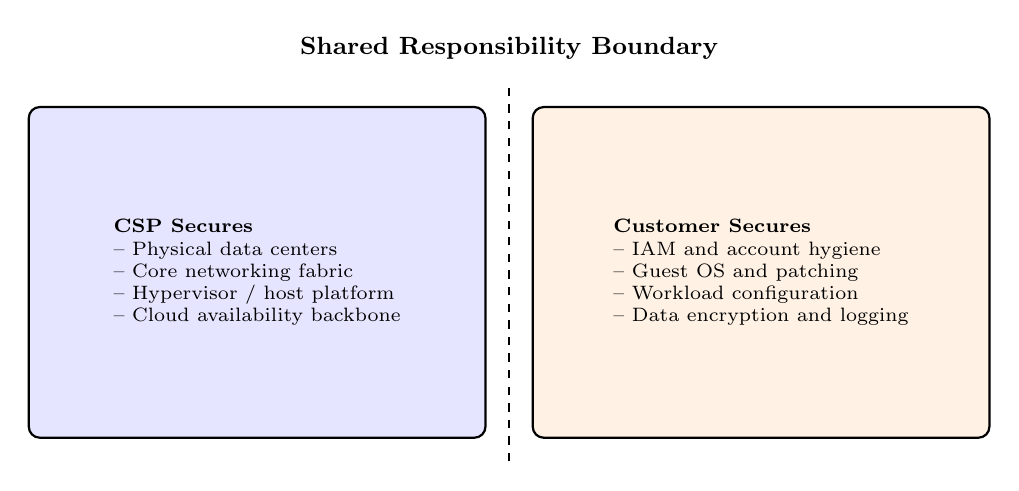
\begin{tikzpicture}[
        block/.style={rectangle, rounded corners, minimum width=5.8cm, minimum height=4.2cm, draw, thick, align=left, font=\scriptsize},
        title/.style={font=\small\bfseries}
    ]
        \node[block, fill=blue!10] (csp) at (-3.2,0) {\textbf{CSP Secures}\\
        -- Physical data centers\\
        -- Core networking fabric\\
        -- Hypervisor / host platform\\
        -- Cloud availability backbone};

        \node[block, fill=orange!10] (cust) at (3.2,0) {\textbf{Customer Secures}\\
        -- IAM and account hygiene\\
        -- Guest OS and patching\\
        -- Workload configuration\\
        -- Data encryption and logging};

        \draw[thick, dashed] (0,-2.4) -- (0,2.4);
        \node[title] at (0,2.85) {Shared Responsibility Boundary};
    \end{tikzpicture}
    \caption{IaaS Shared Responsibility Model in SCDF Context}
    \label{fig:shared_responsibility_scdf}
\end{figure}

This division implies that technical operators must explicitly manage controls ``in the cloud'' (e.g., IAM, logging, encryption), whereas strategic actors govern business risk that is not covered by provider protections. Understanding these boundaries prevents misattribution of responsibility --- a common cause of cloud misconfigurations and security lapses. A well-communicated responsibility model ensures that both management and technical operators have clear expectations about what they must oversee, and what is assumed by their provider, reducing ambiguity in operational workflows and enhancing accountability \citep{Al2023Security}.

% ----------------------------------------------------------
\section{Tooling and Control Mapping}
\label{sec:tooling_mapping}

To operationalize the Secure Cloud Deployment Framework (SCDF), this section presents a structured mapping of security tools and controls aligned with SME priorities and cloud security best practices. Cloud environments are layered and dynamic; tooling must therefore be purpose-built to address configuration risks, identity and access management, network controls, monitoring, and recovery support --- all while remaining accessible to resource-constrained small and medium enterprises \citep{Chen2023Securing,Al2023Security}.

Modern cloud security guidance advocates a multi-layered strategy that incorporates preventive, detective, analytic, and mitigation tools across key security domains \citep{Gibreel2023Factors,Tanimu2023Review}. The tool mapping in SCDF is grounded in continuous security posture management, vulnerability assessment, and scalable monitoring approaches suitable for incremental deployment.


\subsection{Tool Selection Criteria}
\label{subsec:tool_selection_criteria}

Security tooling in SCDF must satisfy the following criteria:

\begin{itemize}
    \item \textbf{Cost Accessibility:} Open-source, freemium, or usage-included services with little to no upfront licensing cost.
    \item \textbf{Complexity Appropriateness:} Deployable and maintainable by generalist IT operators without specialized security expertise.
    \item \textbf{Maintenance Sustainability:} Actively maintained tools with strong community support or vendor reliability.
    \item \textbf{Provider Compatibility:} Functional across major IaaS platforms or available via cloud-native APIs that work with provider-agnostic workflows.
\end{itemize}

These criteria align with practical SME guidance emphasizing that tools must be lightweight yet effective --- striking a balance between security needs and operational constraints \citep{Skafi2020Factors,Wilson2015Enablers}.

\begin{figure}[htbp]
    \centering
    \begin{tikzpicture}[
        crit/.style={ellipse, draw, thick, minimum width=2.8cm, minimum height=1cm, align=center, font=\scriptsize\bfseries, fill=blue!10},
        center/.style={rectangle, rounded corners, draw, thick, minimum width=3.2cm, minimum height=1cm, align=center, font=\small\bfseries, fill=green!15},
        arrow/.style={->, >=stealth, thick}
    ]
        \node[center] (sme) at (0,0) {SME Tooling\\Decision};
        \node[crit] (cost) at (-4,2) {Cost\\Accessibility};
        \node[crit] (complex) at (4,2) {Complexity\\Fit};
        \node[crit] (maint) at (-4,-2) {Maintenance\\Sustainability};
        \node[crit] (compat) at (4,-2) {Provider\\Compatibility};

        \draw[arrow] (sme) -- (cost);
        \draw[arrow] (sme) -- (complex);
        \draw[arrow] (sme) -- (maint);
        \draw[arrow] (sme) -- (compat);
    \end{tikzpicture}
    \caption{SCDF Tool Selection Decision Criteria for SMEs}
    \label{fig:tool_selection_criteria_sme}
\end{figure}

\subsection{Identity and Access Management (IAM)}
\label{subsec:iam_tools}

Identity and Access Management (IAM) forms the foundation of secure cloud operations. Concentric layers of identity controls help prevent unauthorized access, one of the most common vectors in cloud breaches.

\textbf{Core IAM tool categories:}

\begin{table}[htbp]
    \centering
    \caption{SCDF IAM Tooling by Phase}
    \label{tab:iam_tools}
    \resizebox{\textwidth}{!}{%
    \begin{tabular}{|l|l|l|l|l|}
        \hline
        \textbf{Tool/Service} & \textbf{Purpose} & \textbf{Phase} & \textbf{Effort} & \textbf{Cost} \\
        \hline
        Native Cloud IAM & Provider-managed identity and roles & P1 & Low & Included \\
        \hline
        MFA (Native/TOTP) & Multi-factor authentication enforcement & P1 & Low & Free \\
        \hline
        Open-Source IAM (Keycloak) & Centralized authentication and federation & P2 & Medium & OSS \\
        \hline
        ITDR* & Detect \u0026 respond to identity compromise patterns & P3 & Medium & OSS/Freemium \\
        \hline
    \end{tabular}%
    }
\end{table}

*Identity Threat Detection and Response extends basic IAM with behavioral alerting for compromised credentials.

\textbf{Critical Control:} Phase 1 deployment must enforce least privilege and MFA on all privileged access before further controls are introduced to reduce the likelihood of account abuse \citep{Trigueros2024Security}.

\subsection{Network and Edge Protection}
\label{subsec:network_tools}

Network protections restrict exposure to external threats and internal lateral movement.

\begin{table}[htbp]
    \centering
    \caption{SCDF Network Protection Tooling by Phase}
    \label{tab:network_tools}
    \resizebox{\textwidth}{!}{%
    \begin{tabular}{|l|l|l|l|l|}
        \hline
        \textbf{Tool/Service} & \textbf{Purpose} & \textbf{Phase} & \textbf{Effort} & \textbf{Cost} \\
        \hline
        Security Groups / Firewall Rules & Default-deny network boundaries & P1 & Low & Included \\
        \hline
        Network ACLs & Subnet-level traffic filtering & P1 & Low & Included \\
        \hline
        Freemium WAF (Cloudflare) & Application-layer attack prevention & P2 & Low & Freemium \\
        \hline
        VPN / Secure Access (WireGuard) & Secured administrative access & P2 & Low & OSS \\
        \hline
        CASB* & Policy enforcement \u0026 usage visibility & P3 & Medium & OSS/Freemium \\
        \hline
    \end{tabular}%
    }
\end{table}

*A Cloud Access Security Broker (CASB) offers intermediate policy enforcement between users and cloud services, helping enforce identity and data security policies across diverse applications and users \citep{Rashid2024Analysis}.

\textbf{Critical Control:} Phase 1 must implement default-deny security groups for all inbound access, limiting services to minimal necessary ports and protocols.

\subsection{Configuration Hardening and Audit}
\label{subsec:hardening_tools}

Misconfigurations are among the most pervasive cloud security risks; therefore, SCDF prioritizes continuous posture assessment and remediation.

\begin{table}[htbp]
    \centering
    \caption{SCDF Configuration Hardening Tooling by Phase}
    \label{tab:hardening_tools}
    \resizebox{\textwidth}{!}{%
    \begin{tabular}{|l|l|l|l|l|}
        \hline
        \textbf{Tool/Service} & \textbf{Purpose} & \textbf{Phase} & \textbf{Effort} & \textbf{Coverage} \\
        \hline
        CSPM* & Continuous configuration checks & P2 & Medium & Multi-cloud \\
        \hline
        CloudSploit & Misconfiguration discovery \u0026 monitoring & P3 & Low & Multi-cloud \\
        \hline
        Trivy & Container and infrastructure vulnerability scanning & P2 & Low & CI/CD \\
        \hline
        CIS Benchmarks & Hardening standards & P2/P3 & Medium & All IaaS \\
        \hline
        OpenVAS & Vulnerability scanner & P2 & Medium & Multi-scope \\
        \hline
    \end{tabular}%
    }
\end{table}

*CSPM tools continuously scan cloud environments for misconfigurations and compliance risks, addressing latent issues before they lead to exploitation \citep{Gibreel2023Factors}. Regular cloud posture monitoring is a recommended security practice to maintain consistent security baselines and accelerate detection of configuration drift \citep{Al2023Security}.

\textbf{Automation Priority:} Weekly posture scans and drift detection provide early warning and remediation opportunities before incidents occur.

\subsection{Monitoring and Logging}
\label{subsec:monitoring_tools}

Ongoing visibility into events and trends is essential for detecting anomalies and operational issues.

\begin{table}[htbp]
    \centering
    \caption{SCDF Monitoring and Logging Tooling by Phase}
    \label{tab:monitoring_tools}
    \resizebox{\textwidth}{!}{%
    \begin{tabular}{|l|l|l|l|l|}
        \hline
        \textbf{Tool/Service} & \textbf{Purpose} & \textbf{Phase} & \textbf{Effort} & \textbf{Notes} \\
        \hline
        Cloud-native logging & Provider-managed log collection & P1 & Low & Basic logging \\
        \hline
        SIEM / Log Aggregation & Centralized analysis and alerting & P3 & Medium & OSS/Freemium \\
        \hline
        CloudSploit & Supplementary config alerts & P3 & Low & CSPM \\
        \hline
        Graylog / Loki / OpenSearch & Aggregation \u0026 searchable logs & P3 & Medium & OSS \\
        \hline
        Metrics Monitoring & Trend visualization & P3 & Low & OSS \\
        \hline
    \end{tabular}%
    }
\end{table}

A blend of provider-native logging and centralized alerting supports correlation, investigation, and dashboarding. Cloud security monitoring tools significantly enhance situational awareness by collecting logs, correlating alerts, and aiding in incident detection and forensics \citep{Gupta2023Deep}.

\textbf{Monitoring Best Practice:} Configure automated alerts for high-risk events (e.g., failed logins, unexplained privilege escalations) to enable prompt human validation and response.

\subsection{Backup and Recovery}
\label{subsec:backup_tools}

Backup and recovery tools ensure business continuity and resilience.

\begin{table}[htbp]
    \centering
    \caption{SCDF Backup and Recovery Tooling by Phase}
    \label{tab:backup_tools}
    \resizebox{\textwidth}{!}{%
    \begin{tabular}{|l|l|l|l|l|}
        \hline
        \textbf{Tool/Service} & \textbf{Purpose} & \textbf{Phase} & \textbf{Effort} & \textbf{Encryption} \\
        \hline
        Cloud snapshots & VM \u0026 storage backups & P1 & Low & Provider-managed \\
        \hline
        Restic / BorgBackup & Deduplicated, encrypted backups & P4 & Medium & AES-256 \\
        \hline
        Duplicati / Kopia & File-level encrypted backups & P4 & Low & AES-256 \\
        \hline
        Rclone & Sync backups to object storage & P4 & Low & Optional \\
        \hline
    \end{tabular}%
    }
\end{table}

Daily backups with defined retention policies and periodic recovery tests protect against data loss due to misconfigurations, incidents, or outages --- a foundational resilience measure emphasized in cloud risk management practices \citep{Matias2019Cloud,Chan2023Digital}.

\textbf{Resilience Requirement:} Automated backups should occur daily with monthly restoration tests to verify integrity and restore procedures.

\subsection{Vulnerability Assessment and Remediation}
\label{subsec:vulnerability_tools}

\begin{table}[htbp]
    \centering
    \caption{SCDF Vulnerability Management Tooling by Phase}
    \label{tab:vulnerability_tools}
    \resizebox{\textwidth}{!}{%
    \begin{tabular}{|l|l|l|l|l|}
        \hline
        \textbf{Tool/Service} & \textbf{Purpose} & \textbf{Phase} & \textbf{Effort} & \textbf{Coverage} \\
        \hline
        Nessus Essentials / OpenVAS & Vulnerability scanning & P2 & Medium & Host \u0026 network \\
        \hline
        Trivy / Cyera* & Container / IaC scanning & P2 & Low & CI/CD \\
        \hline
        Snyk (Free) & OSS dependency scanning & P2 & Low & Libraries \\
        \hline
    \end{tabular}%
    }
\end{table}

*Container and infrastructure vulnerability scanning.

Continuous vulnerability scanning that prioritizes by exploitability and asset criticality helps SMEs to remediate known exposures before attackers can leverage them \citep{Abdulsalam2023Security}.

\textbf{SLR-Informed Requirement:} Weekly scans of production instances and registries help detect emerging weaknesses that result from software, infrastructure, or configuration changes.

\subsection{Master Tool-to-Phase Mapping}
\label{subsec:tool_mapping_summary}

\begin{table}[htbp]
    \centering
    \caption{SCDF Master Tool-to-Phase Mapping}
    \label{tab:master_tool_mapping}
    \resizebox{\textwidth}{!}{%
    \begin{tabular}{|l|l|l|l|}
        \hline
        \textbf{Phase} & \textbf{Tools/Controls} & \textbf{Core Risk Addressed} & \textbf{Cumulative Effort} \\
        \hline
        \textbf{P1: Baseline} & IAM, MFA, Security groups, basic logging, snapshots & Identity \u0026 network access & Low \\
        \hline
        \textbf{P2: Hardening} & CSPM, CIS Benchmarks, vuln scanners, VPN/WAF & Misconfiguration \u0026 vulnerability exposure & Medium \\
        \hline
        \textbf{P3: Monitoring} & SIEM \u0026 log aggregation, metrics, automated alerts & Anomalous activity \u0026 incident detection & High \\
        \hline
        \textbf{P4: Recovery} & Backups \u0026 recovery tools, continuity testing & Data loss \u0026 continuity risk & Moderate \\
        \hline
    \end{tabular}%
    }
\end{table}

This master mapping enables SMEs to plan and resource SCDF implementation in a structured way, aligning tools with common threat vectors and documented cloud security best practices \citep{Milhem2025integrated,Sabah2024Cloud}.

% ----------------------------------------------------------
\section{IaaS Provider Coverage}
\label{sec:provider_coverage}

This section defines which Infrastructure-as-a-Service (IaaS) providers SCDF is intended to support and why they were selected from both global market and SME usability perspectives. IaaS delivers foundational cloud resources (compute, storage, networking) under a subscription model, allowing organizations to run virtual machines, manage storage, and host applications without owning physical infrastructure. Customers retain control of virtual machine configuration, access policies, and the security of hosted workloads --- which makes strong deployment practices essential \citep{Chen2023Securing}.

\subsection{Dominant Global IaaS Providers}
\label{subsec:dominant_providers}

SCDF prioritizes support for the largest and most widely adopted IaaS providers globally, because these platforms collectively host the majority of SME cloud deployments and offer mature security tool chains that dovetail with the framework's controls:

\begin{itemize}
    \item \textbf{Amazon Web Services (AWS)} --- Recognized widely as a market leader in IaaS with a broad global reach, comprehensive service portfolio, and robust native security controls.
    
    \item \textbf{Microsoft Azure} --- Strong enterprise and SMB adoption, especially where integration with Microsoft ecosystems (e.g., Active Directory, Office 365) is beneficial.
    
    \item \textbf{Google Cloud Platform (GCP)} --- Known for advanced networking, analytics, and security tooling.
    
    \item \textbf{IBM Cloud} --- Used by organizations seeking hybrid cloud architectures or specialized enterprise features.
    
    \item \textbf{Oracle Cloud Infrastructure (OCI)} --- Appeals to SMEs requiring integrated database and application services.
    
    \item \textbf{Alibaba Cloud} --- Competitive in Asia and Middle Eastern markets with strong cost-performance profiles.

    \item \textbf{Additional providers (e.g., Kamatera)} --- Emerging IaaS options that offer flexible VPS and scalable infrastructure, sometimes at lower costs, which can be suitable for SMEs prioritizing simplicity over ecosystem breadth.
\end{itemize}

These providers collectively capture the majority of the public cloud IaaS market and represent platforms where SCDF's risk-based controls and tooling patterns (IAM hardening, posture management, logging) can be directly applied \citep{Al2023Security,Rashid2024Analysis}.

\subsection{SME-Focused and Cost-Efficient Providers}
\label{subsec:sme_providers}

Beyond the major hyperscale cloud vendors, there is a class of cloud providers that are operationally attractive for SMEs due to predictable pricing, simplicity, and ease of onboarding. SCDF is designed to be portable to these environments as well:

\begin{itemize}
    \item \textbf{DigitalOcean} --- Popular with startups and developers for straightforward VPS hosting and predictable pricing.
    
    \item \textbf{OVHcloud} --- Offers flexible infrastructure options and European data-sovereignty advantages.
    
    \item \textbf{Hetzner Cloud} --- Known for cost-effective compute and storage options.
    
    \item \textbf{Linode, Vultr, Scaleway} --- Alternative IaaS options that provide simple cloud servers and networking, often appealing to micro-SMEs or early-stage deployments.
\end{itemize}

These providers may lack some advanced native security services compared to hyperscale vendors, but SCDF's tooling catalog and deployment phases are designed to accommodate environments where provider-native controls may be supplemented by open-source or 3rd-party tools \citep{Skafi2020Factors,Chan2023Digital}.

\subsection{Security Considerations Across Providers}
\label{subsec:cross_provider_security}

While the responsibility for physical infrastructure and host virtualization security lies with the cloud provider, SMEs must secure their own configurations, access controls, and workload protections. The shared responsibility model under IaaS means that:

\begin{itemize}
    \item \textbf{Providers secure:} underlying hardware, network fabric, and virtualization layer.
    \item \textbf{Customers secure:} identity and access, operating systems, application configurations, encryption, and logging.
\end{itemize}

\begin{figure}[htbp]
    \centering
    \resizebox{0.98\textwidth}{!}{%
    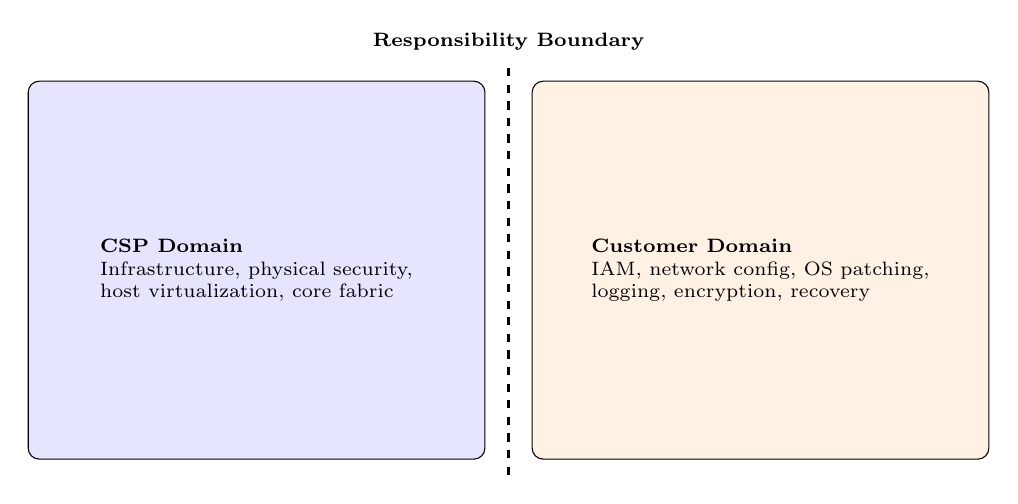
\begin{tikzpicture}[
        box/.style={rectangle, draw, rounded corners, minimum width=5.8cm, minimum height=4.8cm, font=\scriptsize, align=left},
        tag/.style={rectangle, draw=none, fill=white, font=\scriptsize\bfseries, inner sep=2pt}
    ]
        \node[box, fill=blue!10] (csp) at (-3.6,0) {\textbf{CSP Domain}\\
        Infrastructure, physical security,\\
        host virtualization, core fabric};

        \node[box, fill=orange!10] (cust) at (2.8,0) {\textbf{Customer Domain}\\
        IAM, network config, OS patching,\\
        logging, encryption, recovery};

        \draw[thick,dashed] (-0.4,-2.6) -- (-0.4,2.6);
        \node[tag] at (-0.4,2.9) {Responsibility Boundary};
    \end{tikzpicture}%
    }
    \caption{Shared Responsibility Model in IaaS (Provider vs. Customer Domains)}
    \label{fig:shared_responsibility_phase_overlay}
\end{figure}

SCDF assumes this shared model and focuses on the controls that fall within the customer's responsibility domain, ensuring that SMEs can apply standardized security best practices regardless of which IaaS provider they choose. This is consistent with cloud-security best practices that emphasize customer responsibility for OS and configuration level security when using IaaS \citep{AWS2026SharedResponsibilityModel,Microsoft2026SharedResponsibility,Wiz2026SharedResponsibilityModel,Gibreel2023Factors,Trigueros2024Security}.

\subsection{Why These Providers Matter for SCDF}
\label{subsec:provider_rationale}

\textbf{Market Prevalence and Tool Ecosystems:} AWS, Azure, and GCP offer the richest set of security-centric APIs, identity controls, and monitoring services --- enabling more seamless integration with SCDF controls and tooling \citep{Milhem2025integrated}.

\textbf{Operational Flexibility:} SME-oriented providers (DigitalOcean, OVHcloud, etc.) provide simple environments where SCDF's lightweight controls and automation can be deployed without enterprise-grade overhead.

\textbf{Geographic Diversity:} Many SMEs adopt cloud based on regional provider presence and cost considerations. SCDF can adapt to local availability and pricing structures while maintaining core security principles \citep{Sayginer2021Multi,Abdulsalam2023Security}.

Collectively, this coverage ensures that SCDF remains both scalable and relevant across a wide spectrum of SME cloud deployments.

% ----------------------------------------------------------
\section{Evaluation Strategy}
\label{sec:evaluation_strategy}

To assess the effectiveness, suitability, and operational impact of the Secure Cloud Deployment Framework (SCDF) in SME cloud environments, SCDF adopts an evaluation strategy built around measurable, outcome-focused metrics. Rather than relying on qualitative judgments alone, this strategy emphasizes meaningful indicators of security posture, operational overhead, and cost efficiency---particularly for resource-constrained environments \citep{Scrut2022CloudSecurityMonitoring,Olifer2015OntologyMetricsMapping}.

A well-designed evaluation strategy serves several purposes: it provides evidence of security improvement over time, enables justified investment decisions, and supports continuous refinement of controls as threat landscapes evolve.

\subsection{Security Posture Indicators}
\label{subsec:security_posture_indicators}

Security posture indicators are quantitative metrics that reflect an organization's exposure to risk and its ability to detect, prevent, or respond to threats. These metrics should be tracked consistently and compared against established baselines to demonstrate measurable improvement.

Key security posture indicators in SCDF include:

\begin{itemize}
    \item \textbf{Mean Time to Detect (MTTD):} The average time required to detect a security incident after its occurrence. A low MTTD suggests more effective monitoring and visibility \citep{Scrut2022CloudSecurityMonitoring}.
    \item \textbf{Incident frequency:} The number of confirmed security incidents within a defined period (e.g., per quarter), categorized by severity. Consistent reductions over time indicate improved security control effectiveness.
    \item \textbf{Configuration drift percentage:} The proportion of system configurations that deviate from defined secure baselines. This metric helps quantify the effectiveness of automated posture management tools and policy enforcement.
    \item \textbf{Control coverage score:} The percentage of recommended controls implemented and validated versus the total SCDF control set. Progress here demonstrates advancing maturity across SCDF phases.
\end{itemize}

These indicators bridge technical outcomes (such as detection timeliness) with observable improvement patterns that SMEs can benchmark against their baseline.

\subsection{Operational Overhead Metrics}
\label{subsec:operational_overhead_metrics}

Operational overhead metrics measure the cost in time and resources needed to maintain security practices, enabling SMEs to evaluate trade-offs between increased protection and ongoing operational demands. These metrics are essential for demonstrating efficiency---a critical concern for SMEs with limited staff and budget.

Core operational overhead metrics include:

\begin{itemize}
    \item \textbf{Deployment time per phase:} Total elapsed time required to implement each SCDF phase (P1 through P4). These measurements help SMEs plan and allocate resources effectively.
    \item \textbf{Human vs. automation effort ratio:} The proportion of manual operator time relative to automated tasks (e.g., scripted scans, backups). A higher automation share typically indicates increased operational efficiency \citep{Cheenepalli2025DevSecOpsSMEs}.
    \item \textbf{Maintenance time per tool:} Time spent updating and managing each security tool (e.g., CI/CD integration for vulnerability scanning or updating SIEM rules). Documenting this metric supports decisions about tool suitability and cost--benefit trade-offs over time.
\end{itemize}

Operational overhead metrics help SMEs validate that SCDF's phased approach reduces manual workload while improving security outcomes---a key requirement for sustainability in smaller organizations.

\subsection{Cost Efficiency Metrics}
\label{subsec:cost_efficiency_metrics}

Cost efficiency reflects how well security investments (both direct and indirect) produce measurable improvement in security posture without exceeding SME resource capacities. This evaluation dimension ensures SCDF's recommendations remain practical and justifiable from a financial perspective.

Important cost efficiency indicators are:

\begin{itemize}
    \item \textbf{Direct security costs:} Expenses associated with tooling, cloud service consumption (e.g., logging or SIEM usage fees), and any managed services.
    \item \textbf{Indirect efficiency gains:} Indicators such as reductions in incident response time and decreases in manual rework due to automation, which contribute to indirect savings in staff time and lower disruption costs.
    \item \textbf{ROI of security tools:} A ratio comparing security investment to risk reduction or impact avoidance (e.g., costs that would have arisen from typical cloud incidents prevented by SCDF implementation). Quantifying this ROI helps SMEs justify security investments to business leadership.
\end{itemize}

By measuring cost efficiency alongside security posture and operational overhead, SCDF provides a balanced view of security value, allowing SMEs to justify security measures not only technically but financially.

\subsection{Longitudinal Trend Analysis}
\label{subsec:longitudinal_trend_analysis}

Tracking these metrics over time---rather than as one-off snapshots---is critical for demonstrating true improvement and sustainability. By comparing pre-implementation baselines against post-implementation performance at regular intervals (e.g., quarterly reviews), SMEs can:

\begin{itemize}
    \item Assess the impact of each SCDF phase on measurable outcomes.
    \item Identify plateaus or regressions that require remedial planning.
    \item Provide transparent evidence of improvement to stakeholders and decision makers.
\end{itemize}

Longitudinal analysis elevates security evaluation from intuition and checklist completion to data-driven evidence of progress. In this thesis, these metrics are assessed through simulation-based validation and expert evaluation to determine whether SCDF delivers measurable security improvement without prohibitive operational burden.

% ----------------------------------------------------------
\section{Chapter Summary}
\label{sec:chapter3_summary}

This chapter established the Secure Cloud Deployment Framework (SCDF) as a practical, evidence-driven response to the security challenges facing SMEs in developing regions. Key elements defined include:

\begin{itemize}
    \item \textbf{Scope boundaries} that ensure realism through explicit exclusions and a clear target SME profile.
    \item \textbf{Systematic derivation from SLR findings}, mapping documented constraints to actionable framework requirements.
    \item \textbf{Design principles} that prioritise risk-driven, incremental, and automation-assisted security.
    \item \textbf{Layered framework structure} separating governance, controls, and operations into manageable components.
    \item \textbf{Four-phase deployment sequence} ordered by risk reduction per unit effort.
    \item \textbf{Tooling catalogue} mapped to security domains, with all tools satisfying cost and complexity constraints for SMEs.
    \item \textbf{Provider coverage} spanning both dominant hyperscale and SME-focused IaaS platforms.
\end{itemize}

The framework design balances security effectiveness with deployability, recognizing that a framework unimplemented provides no protection regardless of its theoretical completeness. The following chapter validates SCDF through practical implementation scenarios and objective measurement against the evaluation criteria established herein.
